\chapter{Literature Review}

\section{Associative Memory}
Associative memory also known as content addressable memory was first proposed
in the early 1960s by researchers at IBM, including Richard W. Harker, Kenneth
C. Thompson, and Robert D. Denny. CAM is a type of computer memory that allows
for the rapid searching and retrieval of data by using the content of the data
as the address.

In traditional random access memory (RAM), data is stored in a specific
location based on a numerical address and the data can be retrieved by
accessing the corresponding address. In contrast, CAM stores data in a specific
location based on the content of the data and the data can be retrieved by
searching for the specific content rather than the numerical address.

CAM has several advantages over traditional RAM, including faster search and
retrieval times and the ability to store and retrieve data based on the content
rather than a numerical address. These features make CAM particularly useful in
applications where rapid searching and retrieval of data is important, such as
database management and pattern recognition.

The concept of CAM has had a significant impact on the field of computer
science. The work of Harker, Thompson and Denny has contributed to the
development of efficient and effective methods for storing and retrieving data
in computers. Its applications include database management systems which
require searching through the data as fast as possible
figure\ref{associative_circuit} shows one such circuit.
\begin{figure}[h!]
    \centering
    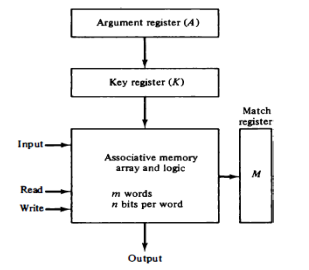
\includegraphics[width=0.7\linewidth]{associative}
    \caption{Associative memory circuit}\label{associative_circuit}
\end{figure}

\section{Associative network}
An associative network is a type of artificial neural network that is designed
to store and retrieve information based on the strength of the connections
between neurons. Associative networks are often used for tasks that require the
recall of specific patterns or relationships, such as image recognition,
natural language processing, and recommendation systems.
\subsection{An Interactive Activation Model of Context Effects in Letter Perception}
\subsubsection{Introduction}
The interactive activation model\cite{auto} is a computational model that
attempts to explain how the brain processes and interprets written language. It
suggests that the brain stores and retrieves information about letters and
words based on the strength of the connections between neurons, and that these
connections are influenced by both bottom-up and top-down processes.

The model proposes that the brain has a hierarchical structure, with
lower-level processing units representing features such as lines and curves,
and higher-level processing units representing letters and words. According to
the model, the activation of a processing unit depends on both the activation
of its inputs and the activation of its outputs.
\subsubsection{Proposed system}
The authors propose a hierarchical structure for the model, with lower-level
processing units representing features such as lines and curves, and
higher-level processing units representing letters and words. They suggest that
the activation of a processing unit depends on both the activation of its
inputs and the activation of its outputs. The main two concepts in this system
are

\begin{description}
    \item[Auto associative memory:]A single layer NN in which the number of training
    vectors and the number of output vectors are the same. The weights are
    determined by the stored patterns.
    \item[Hetero associative memory:]A single layer NN in which the number of input
    training vectors and output are different. Weights are determined by the
    pattern stored in the network. It is static in nature and hence there would be
    no linear or delay operations.
\end{description}
\subsubsection{Advantages }
One advantage of the model is that it provides a computational framework for
understanding how the brain processes and interprets written language. It
suggests a hierarchical structure for the brain, with lower-level processing
units representing features such as lines and curves, and higher-level
processing units representing letters and words. Another advantage of the model
is that it is based on the concept of auto-associative and heteroassociative
memory, which are thought to play a role in perception and language processing
in the human brain. This allows the model to capture the complex relationships
between letters and words, and to explain a wide range of phenomena in written
language processing.

\subsubsection{Disadvantages}
A disadvantage of the model is that it is a simplified model of the brain, and
it may not capture all the complexity and nuance of language processing. It is
also based on a set of assumptions and simplifications, and it may not
accurately reflect the underlying mechanisms of the brain. In addition, the
model is based on a set of equations and learning rules that are used to
simulate the activation and deactivation of processing units, and these
equations may not accurately reflect the underlying mechanisms of the brain.

\subsection{Neural networks and physical systems with emergent collective computational abilities.}
\subsubsection{Introduction}
The Hopfield model\cite{hopfield} is a type of RNN that is designed to mimic
the behaviour of neurons in the brain. It is a type of associative memory
system and hence it can store and recall information based on the relationship
between the data stored. It has applications including pattern recognition,
optimization, and error correction.
\subsubsection{Methodology}
This paper discusses the use of computational models and simulations to study
the behaviour of neural networks and other distributed systems. He proposed an
associative memory network type called the Hopfield network. A Hopfield network
consists of a set of interconnected neurons that are arranged in a single
layer. Each neuron is fully connected in the network, and the connections
between neurons are adjusted based on the strength of the relationships between
the inputs and outputs. The behaviour of a Hopfield network is determined by a
set of equations that describe the activation and deactivation of the neurons
over time. These equations are based on the concept of auto-associative memory,
in which the output is used to retrieve the original input.
\subsubsection{Advantages}
One advantage of the Hopfield model is that it is relatively simple and easy to
implement. It consists of a single layer of interconnected neurons and the
connections between neurons are adjusted based on the strength of the
relationships between the inputs and outputs. This simplicity makes the
Hopfield model easy to understand and implement. Another advantage of the
Hopfield model is that it is capable of storing and retrieving patterns or
sequences of data based on the strength of the connections between neurons.
This makes it useful for tasks that require the recall of specific patterns or
sequences of data, such as image recognition, natural language processing, and
recommendation systems. Also, this model is relatively robust and resistant to
noise. These advantages make it useful in applications like image or speech
recognition systems.
\subsubsection{Disadvantages}
One disadvantage of the Hopfield model is that it is relatively simple and may
not be able to capture the complexity and nuance of more advanced neural
networks. Another drawback is that it can retrieve the information only with
the original input. A third disadvantage of the Hopfield model is that it can
be sensitive to initialization and may not always converge to a stable state
when used with a large amount or insufficiently distinct data. This can make it
difficult to use the model for certain types of tasks, such as optimization or
decision-making.
\section{Spiking neural network}
Spiking neural networks are a type of neural network that models the behaviour
of biological neurons by using spikes or pulses to encode and transmit
information. They are a relatively new type of neural network that has the
potential to improve the performance and efficiency of artificial intelligence
systems. The use of spiking neural networks for building associative memory
systems is a relatively new area of research that has only recently started to
gain attention.

\subsection{SWAT: a spiking neural network training algorithm for classification problems.}
\subsubsection{Introduction}
SWAT\cite{swat}(Spiking Weight association Training) is a method for training
spiking neural networks for classification tasks. It uses a combination of
supervised and unsupervised learning to improve the performance of SNN. It is
based on the idea of adjusting the weights of the connections between neurons
in the network based on the input and output patterns of the network. The
weights are adjusted using a learning rule that takes into account the error
between the actual output of the network and the desired output.
\subsubsection{Methodology}
They propose a method which merges Bienenstock-Cooper-Munro learning rule
(BCM)\cite{bcm} with Spike Time Dependent plasticity Spike-timing-dependent
plasticity (STDP)\cite{stdp}. It yields an unimodal weight distribution where
height is associated with STDP.

The BCM learning rule is based on the idea that the strength of the connections
between neurons in the network should be adjusted based on the activity of the
neurons and the error between the actual output of the network and the desired
output. The rule specifies that the weights of the connections between neurons
should be increased if the activity of the neurons is high and the error is
also high, and the weights should be decreased if the activity of the neurons
is low and the error is also low.

STDP is an unsupervised learning rule based on the functioning of neurons in
the brain for neuromorphic computing, which is the study inspired by the
structure and functioning of the brain. In the process strength of the
connection between neurons changes based on the relative timing of spikes or
impulses The basic idea behind STDP is that if two $N_{pre}$ and $N_{suc}$
neurons are connected, and their spike time are $t_1$ and $t_2$ respectively
according to STDP \vspace*{-.3pc}
\begin{itemize}
    \item[]Weight of connection from $N_{pre}$ to $N_{suc}$ should  increase, if {\boldmath$t_1>t_2$}
    \item[]Weight of connection from $N_{pre}$ to $N_{suc}$ should  decrease, if {\boldmath$t_1<t_2$}
    \item[]Weight of connection from $N_{pre}$ to $N_{suc}$ should  remain same, if {\boldmath$t_1=t_2$}

\end{itemize}
%\vspace*{-2pc}

Overall SWAT is based on the idea of adjusting the weights of the connections
between neurons in the network based on the input and output patterns of the
network. The weights are adjusted using a learning rule that takes into account
the error between the actual output of the network and the desired output.
\subsubsection{Advantages}
One of the main advantages of SWAT is that it can be used to train spiking
neural networks for classification tasks. This is important because spiking
neural networks are a promising type of artificial neural network that is
thought to have the potential to improve the performance of artificial
intelligence systems. It uses a combination of supervised learning and
unsupervised learning to train the network. This allows the network to learn
from labelled examples as well as identify patterns and features in the data on
its own. Since it is based on the simple learning rules of adjusting the
weights of the connections between neurons in the network based on the input
and output patterns of the network it is relatively easy to implement and
understand. Overall it has the potential to enable the use of SNN in a wide
range of applications.
\subsubsection{Disadvantages}
Sometimes this may become computationally intensive, especially for large
networks with many neurons and connections. This could make it difficult to use
SWAT on systems with limited computational resources. Another potential
disadvantage is that it is based on supervised and unsupervised learning, in
which supervised learning requires a large amount of labelled data to train the
network effectively. This may be difficult to obtain in some cases. It also
relies on the initial weights of the connections between neurons in the
network, and these weights may have a significant impact on the performance of
the network. This means that SWAT may be sensitive to initialization and may
require careful tuning of the initial weights to achieve good performance.
\subsection{SpikeProp: backpropagation for networks of spiking neurons.}
\subsubsection{Introduction}
Spiking neurons may be more biologically realistic and efficient than other
types of artificial neurons, and they may be more suitable for certain tasks
such as pattern recognition and natural language processing. However, they also
note that training networks of spiking neurons can be difficult due to the
non-differentiable nature of the spiking function. To address this problem, the
authors propose the use of SpikeProp\cite{spikeprop}, which is a method for
training networks of spiking neurons using backpropagation.
\subsubsection{Methodology}
It is a method for training networks of spiking neurons using backpropagation.
The spiking function, which describes the relationship between the input and
the output of a spiking neuron, is not differentiable. This means that
traditional methods for training artificial neural networks, such as
backpropagation, cannot be directly applied to networks of spiking neurons.This
can be avoided by surrogate gradient function that approximates the gradient of
the spiking function, which allows the use of backpropagation to train networks
of spiking neurons.

\subsubsection{Advantages}
It allows the use of backpropagation to train networks of spiking neurons. This
makes it possible to leverage the simplicity and efficiency of backpropagation
for training spiking neural networks. With spikeprop, it is possible to create
artificial neural networks that are more biologically realistic and may be more
suitable for certain tasks. It is also more efficient in training SNN than
other techniques. It makes it effective in applications like image recognition
and language translation.
\subsubsection{Disadvantages}
It is not effective in all applications of spiking neural networks. Also, due to
the approximations used in surrogate gradient function, it may not be always
accurate which may affect its performance.